\chapter{Cross-Site Request Forgery}

Gli attacchi CSRF (Cross-Site Request Forgery) sfruttano il modo in cui operano i browser e la relazione di fiducia tra un sito Web e il browser.\\

Individuando le chiamate API che si basano su questa relazione per garantire la sicurezza, possiamo creare  collegamenti e moduli che, con un piccolo sforzo, possono indurre un utente a effettuare richieste per proprio conto (sfruttando i \textbf{cookie di sessione} locali) ma alla sua insaputa.\\

I due principali identificatori di un attacco CSRF sono:
\begin{itemize}
	\item Privilege escalation 
	\item L'account utente che avvia la richiesta solitamente non si accorge di nulla (è un attacco furtivo)	
\end{itemize}

\section{Le richieste GET - Esempio}
Solitamente l'attacco sfrutta le richieste HTTP GET e per farlo procede così:
\begin{itemize}
	\item Un hacker scopre che un server web utilizza richieste HTTP GET per modificare il suo flusso logico (ad esempio, in questo caso, determinando la logica, l'importo e l'obiettivo di un bonifico bancario).
	\item L'hacker crea una stringa URL con questi parametri:\\ \verb|<a href="https://www.mega-bank.com/transfer?to_user=|\\
	\verb|<account dell'hacker>&amount=10000">cliccami</a>.|
	\item L'hacker sviluppa una strategia di distribuzione: di solito è 
	mirata verso chi ha la più alta probabilità di avere già una \textbf{sessione aperta} con la propria banca, o a chi ha molti soldi, o tramite semplice distribuzione di massa sperando di colpire il maggior numero di persone in un breve periodo di tempo prima che l'attacco venga rilevato.
\end{itemize}

\begin{figure}[H]
	\centering
	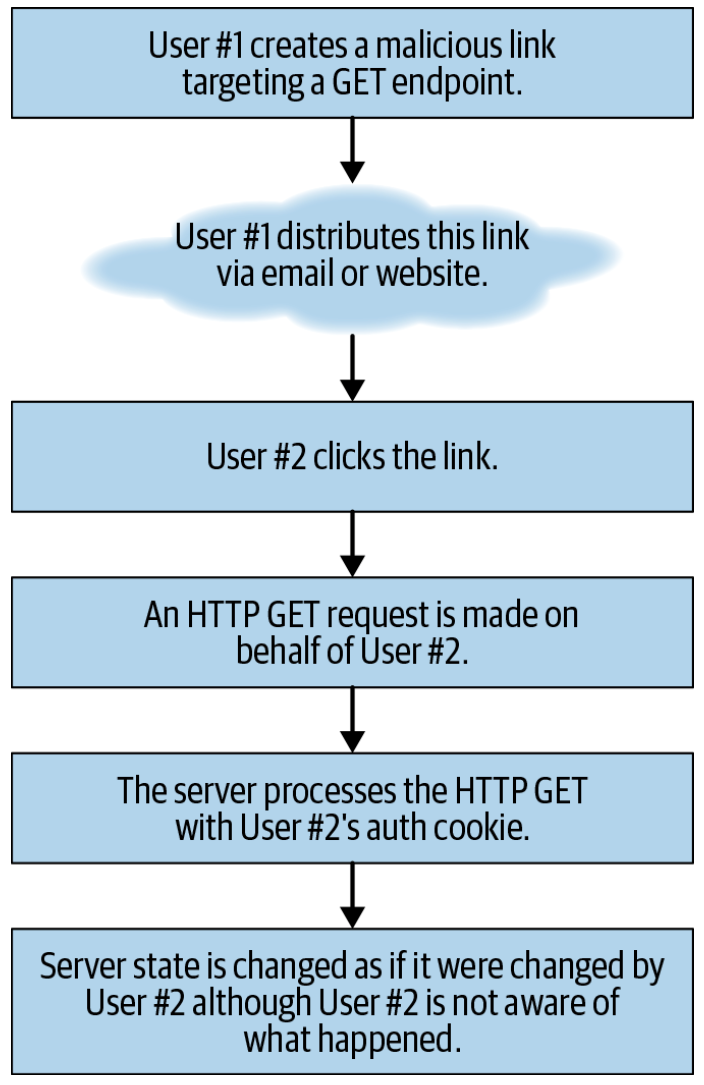
\includegraphics[width=7cm, keepaspectratio]{capitoli/web_security/imgs/get_flow.png}
	\caption{Flow attacco CSRF sfruttando richiesta GET.}
\end{figure}

In Figura~\ref{fig:csrf_banca} possiamo vedere un esempio pratico di attacco. Inizialmente si ha che l'attaccante crea un proprio sito su cui inserisce il tag HTML delle immagini per far caricare automaticamente una risorsa. Però, invece di metterci l'url di una foto, inserisce il \textbf{payload} ovvero una richiesta (GET) di trasferimento soldi dal conto di una banca (su cui spera che l'utente abbia una sessione attiva) presso il proprio conto. Se poi l'attaccante, tramite del \textbf{social engineering}\footnote{Phishing o meglio ancora Spear Phishing.}, riesce a far cliccare la vittima sul proprio link e a reindirizzarla sul proprio sito, ecco che l'attacco avrà buona probabilità di funzionare.

\begin{figure}[H]
	\begin{subfigure}{1\textwidth}
		\centering
		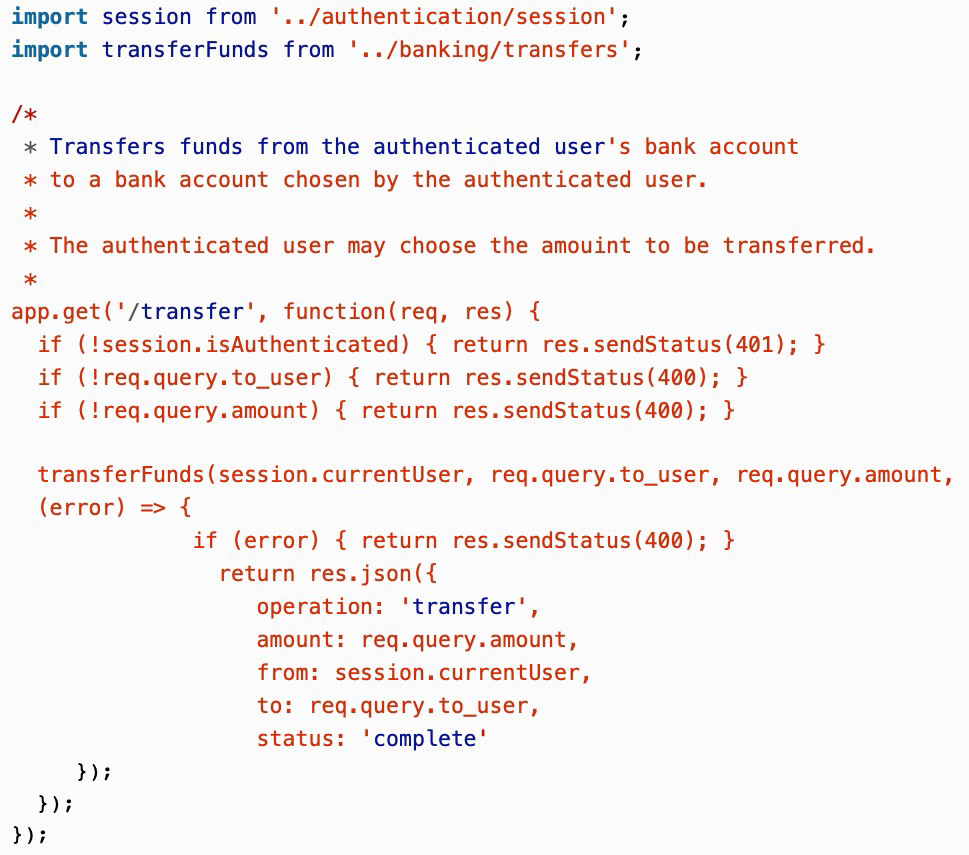
\includegraphics[width=12cm]{capitoli/web_security/imgs/csrf_banca_1.png}  
		\caption{Backend banca.}
		\label{fig:csrf_banca_1}
	\end{subfigure}
	
	\vspace{1.5em}
		
	\begin{subfigure}{1\textwidth}
		\centering
		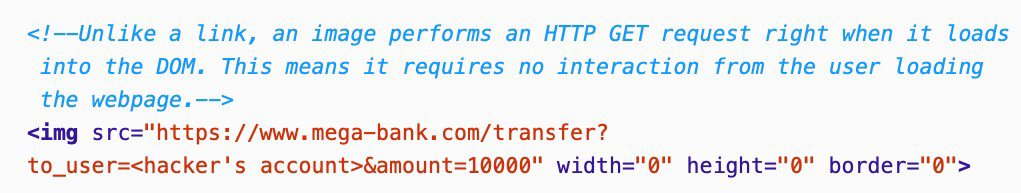
\includegraphics[width=12cm]{capitoli/web_security/imgs/csrf_banca_2.png}  
		\caption{Backend attaccante.}
		\label{fig:csrf_banca_2}
	\end{subfigure}
	\caption{Esempio attacco CSRF banca.}
	\label{fig:csrf_banca}
\end{figure}

\newpage

\section{Le richieste POST}

In genere gli attacchi CSRF avvengono contro gli endpoint GET poiché è molto più facile distribuire un CSRF tramite un collegamento ipertestuale, un'immagine o un altro tag HTML che avvia automaticamente una richiesta. Tuttavia, è possibile inviare un payload CSRF mirato a un endpoint POST, PUT o DELETE. Ciò però risulta più complesso in quanto il payload POST richiede un'interazione obbligatoria con l'utente.\\

Quando l'attacco viene effettuato tramite richieste
POST, solitamente si sfruttano i moduli del browser e in particolare l'oggetto HTML \textbf{<form></form>} che è uno dei pochi in grado di avviare una richiesta POST senza
che sia necessario alcuno script.\\

L'oggetto \textbf{form} inoltre, per sua caratteristica, permette di utilizzare dei campi nascosti (``hidden'') che non vengono mostrati a schermo ma che vengono inclusi al momenti della richiesta. Nell'esempio seguente infatti possiamo notare come i campi ``to\_user'' e ``amount'' siano di tipo ``hidden'' così che la vittima non li possa notare ma così facendo, quando l'utente cliccherà sul pulsante di invio modulo, verranno inclusi nella richiesta dando il via all'attacco e quindi al trasferimento dei suoi soldi sul conto dell'hacker.

\begin{figure}[H]
	\centering
	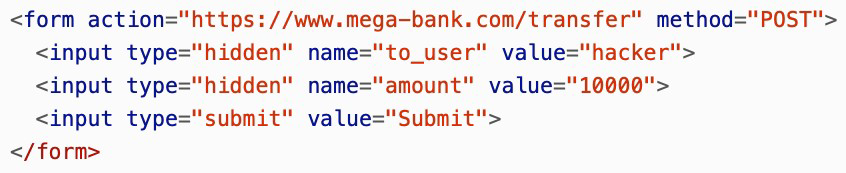
\includegraphics[width=12cm, keepaspectratio]{capitoli/web_security/imgs/csrf_banca_3.png}
	\caption{Backend attaccante.}
	\label{fig:csrf_banca_3}
\end{figure}

Tale attacco è molto utile anche per accedere alle \textbf{reti interne}. Infatti il creatore di un modulo non può fare richieste ai server di una rete interna, ma se un utente che si trova sulla rete interna compila e invia il modulo, la richiesta verrà fatta al server interno come risultato dell'accesso elevato alla rete dell'utente di destinazione. 

\begin{figure}[H]
	\centering
	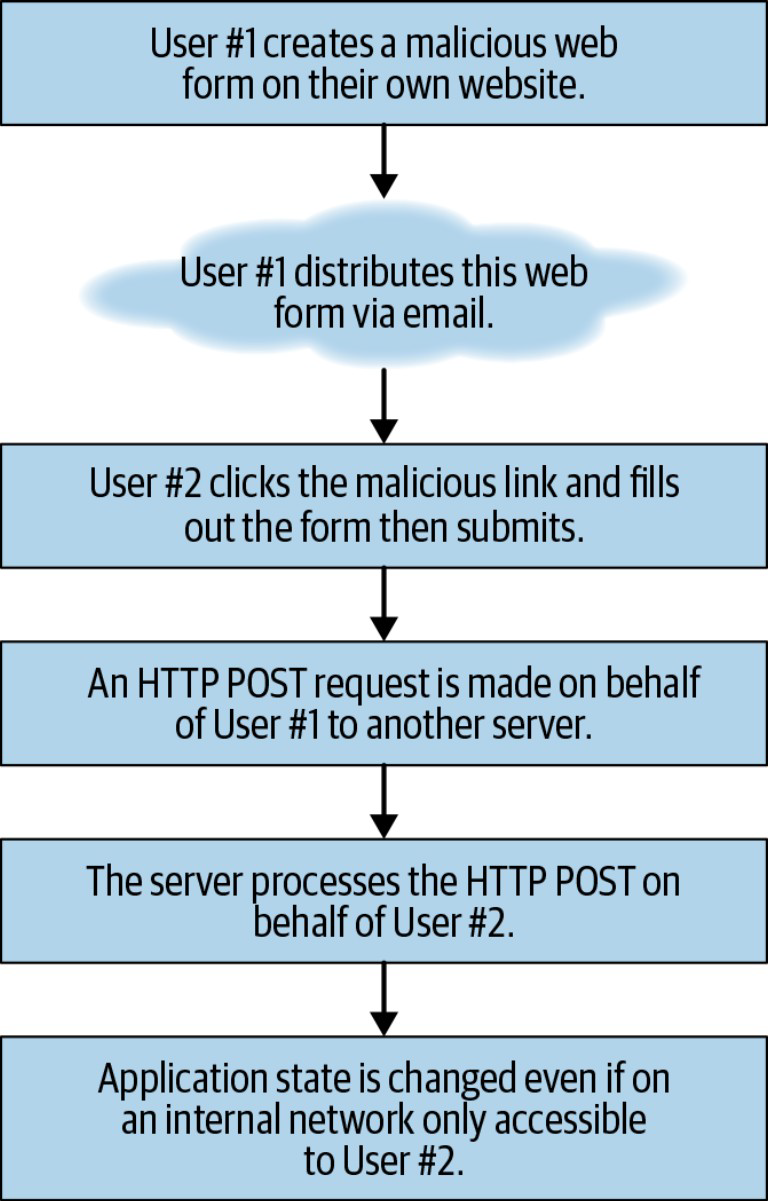
\includegraphics[width=7cm, keepaspectratio]{capitoli/web_security/imgs/post_flow.png}
	\caption{Flow attacco CSRF sfruttando richiesta POST.}
\end{figure}